\section{Analysis method}
\subsection{Measurement Strategy -- TPC "slicing"}
\label{sec:KXSStrategy}
A thin target is a target formed by a slab of material containing many uniformly distributed diffusion centers, where  one center is not sitting in front of another. In this approximation, the survival probability of a kaon traveling through a slab of argon of depth {\it z} and density {\it n} is given by:

\begin{equation}
P_{surv} = e^{-\sigma_{tot}n z}
\end{equation} 
where $\sigma_{tot}$ is the total cross section per nucleon (in $cm^2$), {\emph{z}} is the target thickness (in cm) along the incident kaon direction, and {\emph{n}} is the scattering center density in the target, $n=\frac{\rho N_{A} }{A}$ (in $cm^{-3}$). Thus, the interaction probability is $P_{int} = 1 - P_{surv}$. $P_{int}$ is experimentally measured as the ratio of the number of interacting kaons $N_{int}$ over the number of incident kaons $N_{inc}$:
\begin{equation}
P_{int}=\frac{N_{int}}{N_{inc}}=1-e^{-\sigma_{tot}n z}.
\end{equation}

The assumption of thin target implies $z\rightarrow\delta z$. Thus, it is possible to Taylor expand the exponential and  solve for the total cross section as a function of energy, $\sigma_{tot}(E)$:
\begin{equation}\label{calc_sigma1}
\frac{N_{int}}{N_{inc}}=1-e^{-\sigma_{tot}n z}\simeq 1-(1-\sigma_{tot}n\delta z + o(\delta z^2)) 
\end{equation}
\begin{equation}\label{calc_sigma}
\sigma_{tot}(E) \simeq \frac{1}{n\delta z} \Big(\frac{N_{int}}{N_{inc}}\Big) \text{ 	when $z\rightarrow\delta z$}.
%N_{int}(z,E)=(1-N_{inc}e^{-\sigma_{tot}(E)nz})
\end{equation}


LArIAT, with its 90-cm thick active volume, is not a thin target. Nevertheless, the combination of fine-grained tracking and precise calorimetric information allow us to treat the active volume as a sequence of 240 adjacent thin targets. This technique, called the "sliced TPC" method, allows to measure the kaon cross section as a function of energy.  In LArIAT, the two wire planes are each made of 240 wires oriented at +/- $60^{\circ}$ with a wire pitch of 4 mm; these planes collect signals proportional to the energy loss of the kaon in a $60^{\circ}$-inclined 4~mm thin slab of liquid argon. One can thus think of the TPC as being divided into $\sim$240 slices along the direction of the incident particles ({\emph{z}} axis) with a spacing $\Delta${\emph{z}} = 4 mm/sin($60^{\circ}$) $\approx$ 4.5~mm, as shown in Fig.~\ref{fig:slicedtpc}. Each slice can be now considered a "thin target" and the cross section calculation in Eq.~\ref{calc_sigma} can be iteratively applied. It is possible to perform a differential cross section measurement as a function of the energy because the kaon kinetic energy $K.E._{slice}$  at the beginning of slice is known per each slice. The kaon kinetic energy entering the TPC is determined by measuring the particle momentum with the tertiary beamline and assuming the kaon mass as mass hypothesis. At each slice, the incident energy of the kaon is determined by subtraction of the calorimetric energy released by the particle in the previous slice.\\ 
When the particle enters a slice, it contributes to $N_{inc}$ in the energy bin corresponding to its kinetic energy in that slice. If it interacts in the slice, it also contributes to $N_{int}$ in the appropriate energy bin.\\

An important difference between the thin target approximation and the thick target case needs to be address. While in the first case, only the K-nucleus hadronic interactions are taken into account, other processes such as kaon decay, both in flight and at rest play an important role in the "thick" target case. Kaon decays are a physical background for this measurement. Kaon decay proceeds by the weak interaction; if one only considers the endpoint of the primary kaon track without identification of the decay, this process can be misidentified as a single strong interaction. Kaon decay tagging is discussed the next section. 


%\textcolor{blue}{Sketch of sliced tpc technique?}
\begin{figure}[htpb]
\centering
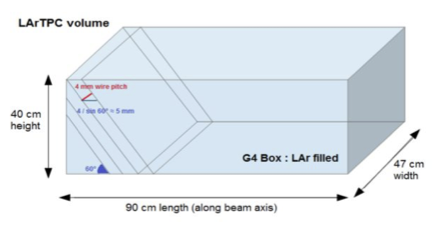
\includegraphics[scale=1.25]{images/Lariat/SlicedTPC.png}\\
\caption{Sketch of Sliced TPC approach.}
\label{fig:slicedtpc}
\end{figure}

